\documentclass[11pt,a4paper]{article}
\usepackage{amsmath,amsthm,amsfonts,amssymb,amscd}
\usepackage{enumerate} 
\usepackage{physics}
\usepackage{enumerate}
\usepackage{fancyhdr}
 \usepackage{hyperref}
\hypersetup{colorlinks,
    linkcolor=blue,
    citecolor=blue,      
    urlcolor=blue,
}
\usepackage{graphicx}


\oddsidemargin0.1cm 
\evensidemargin0.8cm
\textheight22.7cm 
\textwidth15cm \topmargin-0.5cm

\newtheorem{theorem}{Theorem}[section]
\newtheorem{lemma}[theorem]{Lemma}

\usepackage{listings}
\usepackage{xcolor}

\definecolor{codegreen}{rgb}{0,0.6,0}
\definecolor{codegray}{rgb}{0.5,0.5,0.5}
\definecolor{codepurple}{rgb}{0.58,0,0.82}
\definecolor{backcolour}{rgb}{0.95,0.95,0.92}

\lstdefinestyle{mystyle}{
    backgroundcolor=\color{backcolour},   
    commentstyle=\color{codegreen},
    keywordstyle=\color{magenta},
    numberstyle=\tiny\color{codegray},
    stringstyle=\color{codepurple},
    basicstyle=\ttfamily\footnotesize,
    breakatwhitespace=false,         
    breaklines=true,                 
    captionpos=b,                    
    keepspaces=true,                 
    numbers=left,                    
    numbersep=5pt,                  
    showspaces=false,                
    showstringspaces=false,
    showtabs=false,                  
    tabsize=2
}

\lstset{style=mystyle}

\newcommand{\silvia}[1]{{ {\color{blue}{(silvia)~#1}}}}
\newcommand{\grace}[1]{{ {\color{purple}{(grace)~#1}}}}

\newcommand{\MultiSet}{\mathrm{MultiSet}}
\newcommand{\len}{\mathrm{len}}
\newcommand{\din}{\texttt{d\_in}}
\newcommand{\dout}{\texttt{d\_out}}
\newcommand{\T}{\texttt{T} }
\newcommand{\F}{\texttt{F} }
\newcommand{\Relation}{\texttt{Relation}}
\newcommand{\X}{\mathcal{X}}
\newcommand{\Y}{\mathcal{Y}}
\newcommand{\True}{\texttt{True}}
\newcommand{\False}{\texttt{False}}
\newcommand{\clamp}{\texttt{clamp}}
\newcommand{\function}{\texttt{function}}
\newcommand{\float}{\texttt{float }}
\newcommand{\questionc}[1]{\textcolor{red}{\textbf{Question:} #1}}


\title{Privacy Proofs for OpenDP: Is\_Equal Transformation}
\author{Grace Tian}
\date{Summer 2021}
\begin{document}


\maketitle
\tableofcontents

\section{Algorithm Implementation}
\subsection{Code in Rust}
The current OpenDP library contains the \texttt{make\_is\_equal} function implementing the is\_equal function. This is defined in lines 62-71 of the file \texttt{manipulation.rs} in the Git repository (\url{https://github.com/opendp/opendp/blob/21-impute/rust/opendp/src/trans/manipulation.rs#L62-L71}).

\subsection{Code}

%\textbf{OLD:}
%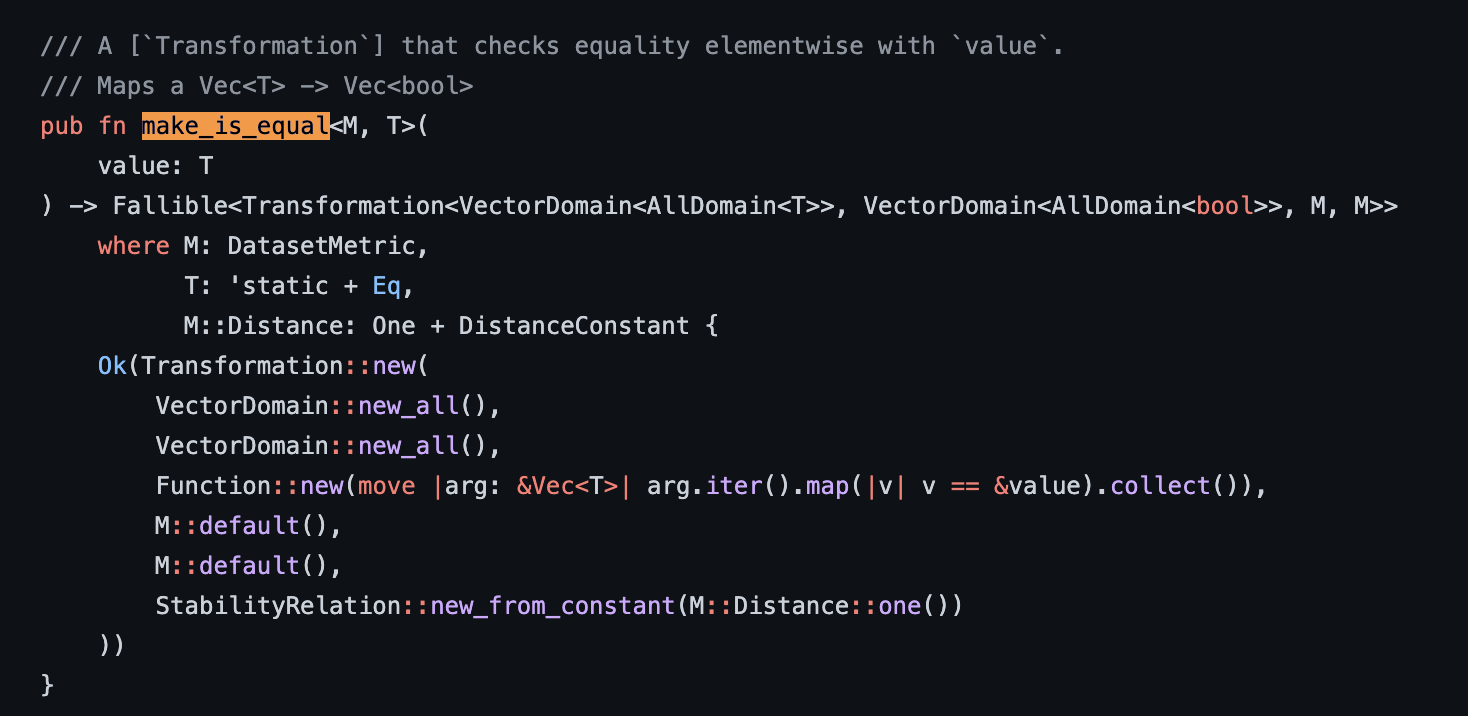
\includegraphics[width=0.8\textwidth]{make_is_equal.png}

%\textbf{NEW:}
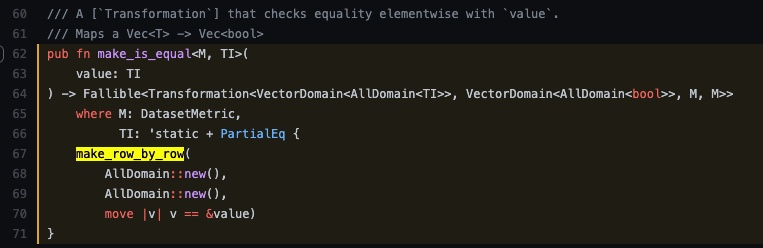
\includegraphics[width=\textwidth]{make_is_equal_new.jpg}


\subsection{Pseudo Code in Python}\label{sec:pseudocode}

\subsubsection*{Preconditions}
To ensure the correctness of the output, we require the following preconditions:

\begin{itemize}
    \item \textbf{User-specified types:}
    \begin{itemize}
        \item Variable \texttt{\texttt{value}} must be of type \texttt{TI}
        \item Type \texttt{T} must have trait \texttt{PartialEq}
    \end{itemize}
\end{itemize}

\subsubsection*{Postconditions}

\begin{itemize}
    \item Either a valid \texttt{Transformation} is returned or an error is returned.
\end{itemize}

\begin{lstlisting}[language=Python, escapechar=|]
def make_is_equal(value : TI):
    input_domain = (VectorDomain(AllDomain(T));
    output_domain = (VectorDomain(AllDomain(bool));
    input_metric = SymmetricDistance(); 
    output_metric = SymmetricDistance();
    
    
    def Relation(d_in: u32, d_out: u32) -> bool: |\label{line:rel}|
        return d_out >= d_in*1
        
    def function(data: Vec(TI)) -> Vec(Bool): |\label{line:fn}|
        return list(map(data == value)) |\label{line:map}|

    return Transformation(input_domain, output_domain, function, input_metric, output_metric, Relation)
\end{lstlisting}

\grace{ For the next round of the updates, will need to change pseudocode so that it returns the result of a make row by row transformation (which the code does). }

\subsection{Proof}
\begin{theorem}


For every setting of the input parameters \texttt{value} to \texttt{make\_is\_equal} such that the given preconditions hold, the transformation returned by \texttt{make\_is\_equal} has the following properties:
\begin{enumerate}
    \item \textup{(Appropriate output domain).} If vector $v$ is in the \texttt{input\_domain}, then \texttt{function(v)} is in the \texttt{output\_domain}.
    \item \textup{(Domain-Metric Compatibility).} The domain \texttt{input\_domain} matches one of the possible domains listed in the definition of \texttt{input\_metric}, and likewise \texttt{output\_domain} matches one of the possible domains listed in the definition of \texttt{output\_metric}.
    \item \textup{(Stability Guarantee).} For every pair of elements $v, w$ in \texttt{input\_domain} and for every pair $(\din, \dout)$, where $\din$ is of the associated type for \texttt{input\_metric} and $\dout$ is the associated type for \texttt{output\_metric}, if $v,w$ are $d_{in}$-close under \texttt{input\_metric} and $\Relation(\din, \dout) = \True$, then $\function(v), \function(w)$ are $d_{out}$-close under \texttt{output\_metric}.
\end{enumerate}
\end{theorem}
\begin{proof}
\begin{enumerate}
\item \textbf{(Appropriate output domain).} The $\function(v)$ has type \texttt{Vec(TI)} follows from the assumption that element $v$ is in \texttt{input\_domain} and from the type signature of \texttt{function} in line~\ref{line:fn} of the pseudocode (Section~\ref{sec:pseudocode}), which takes in an element of type \texttt{Vec(TI)} and returns an element of type \texttt{Vec(Bool)}. If the Rust code compiles correctly, then the type correctness follows from the definition of the type signature enforced by Rust. Otherwise, the code raises an exception for incorrect input type. 

\item \textbf{(Domain-metric compatibility).} 

Symmetric distance is compatible with \texttt{VectorDomain(AllDomain(TI))} for any generic type \texttt{TI}, as stated in \href{https://www.overleaf.com/project/60d215bf90b337ac02200a99}{``List of definitions used in the pseudocode"}. The theorem holds because for \texttt{make\_is\_equal}, the input domain is \texttt{VectorDomain(AllDomain(TI))} for generic type \texttt{TI} and the output domain is \texttt{VectorDomain(AllDomain(bool))}. 

\item \textbf{(Stability guarantee).} 
Because $\Relation(\din, \dout) = \texttt{True}$, it follows that $\din \leq \dout$ by the \texttt{is\_equal} stability relation defined in the pseduocode.

Since vector inputs $v, w$ are $\din$-close, then the symmetric distance is bounded by $\din$ by definition the symmetric distance is bounded by $d_{in}$: $d_{Sym}(v, w) \leq \din$.

We apply the histogram notation, as stated in \href{https://www.overleaf.com/project/60d215bf90b337ac02200a99}{``List of definitions used in the pseudocode"}, to rewrite the symmetric distance in terms of elements $z$ in $\texttt{function}(v)$ and $\texttt{function}(w)$
$$d_{Sym}(v, w) = \norm{h_v - h_w}_1 = \sum_{z} \abs{h_v(z) - h_w(z)}.$$ 

We now want to bound the symmetric distance of the transformed vectors:

$$d_{Sym}(\function(v), \function(w)) = \sum_z \abs{h_{\function(v)}(z) - h_{\function(w)}(z)}.$$

Since each function maps each element to boolean $\{ \T, \F\}$, we consider both cases. 
\begin{enumerate}
    \item $z = \T$:\\
    $$\abs{h_{\function(v)}(\T) - h_{\function(w)}(\T)} = \abs{h_v(\texttt{value}) - h_w(\texttt{value})}$$
    
    \item $z = \F$:\\
    
    Since any element $z \neq \texttt{value}$ maps to \F by definition of \texttt{is\_equal}, we consider all elements $z \neq val$:
    $\abs{h_{\function(v)}(\F) - h_{\function(w)}(\F)} = \abs{\sum_{z \neq val} h_v(z) - h_w(z)}$
    
    By triangle inequality, we have 
    $$\abs{h_{\function(v)}(\F) - h_{\function(w)}(\F)} \leq \sum_{z \neq val} \abs{h_v(z) - h_w(z)}$$
\end{enumerate}


Therefore, we can apply the first two cases respectively to the third line below. 

\begin{align*}
    d_{Sym}(\function(v), \function(w)) &= \sum_z \abs{h_{\function(v)}(z) - h_{\function(w)}(z)} \\
    &= \abs{h_{\function(v)}(\T) - h_{\function(w)}(\T)} + \abs{h_{\function(v)}(\F) - h_{\function(w)}(\F)} \\ 
    &\leq \abs{h_{v}(\texttt{value}) - h_{w}(\texttt{value})} + \sum_{z \neq \texttt{value}} \abs{h_{v}(z) - h_{w}(z)}\\
    &= \sum_z \abs{h_{v}(z) - h_{w}(z)} \\
    &= d_{Sym}(v, w)
\end{align*}

Since $d_{Sym}(\function(v), \function(w)) \leq d_{Sym}(v, w) \leq \din$ and $\din \leq \dout$, it follows that the transformations are \dout-close: $d_{Sym}(\function(v), \function(w)) \leq \dout$.
\grace{TODO in the next round of edits, will use Salil's suggested proof outline with row by row transformation abstraction. This will get rid of casework?}


\end{enumerate}
\end{proof}

\end{document}
